
Nesse capítulo, será apresentada a construção do operador grosso Multiescala. O grid original do problema que se deseja realizar sera denominado grid fino devido os seus elementos serem de menor e o operador associado a esse grid $K^h$ será chamado de operador fino. A partir do grid fino será construido um grid grosso onde cada elemento é uma aglomeração de elementos do grid fino, o operador associado a esse grid será chamado de operador grosso $K^H$.


O método \textit{Multiscale Finite Element Method} (MSFEM) foi introduzido por \citet{thomashou} e inicialmente foi aplicado para obter soluções aproximadas do grid fino através do grid grosso para casos de transferência de calor de materiais e meios porosos com propriedades aleatórias. Algumas da conclusões desses trabalhos foram que o método MSFEM foi capaz de reproduzir a solução da heterogeneidade através da construção das funções de base com solução de problemas locais baseados no operador também que, apesar da construção das bases serem custosas elas podem ser construídas elas podem ser paralelizadas pois são independentes.  Mais tarde, o método MSFEM se mostrou problemático para conservação de massa em problemas de fluxo e por isso foi criado os métodos \textit{Mixed Multiscale Finite Element} (MMSFEM) em \citet{mixedmsfem} e  \textit{Multiscale Finite Volume Method} (MSFVM) em \citet{msfv}.

Apesar do método MSFV garantir a conservação da massa, foi confirmado que em certas situções não se mostrou adequado, dessa forma, foi apresentado o método multiescala iterativo em \citet{iterativems} que ao invés de realizar uma aproximação para a simulação fina utiliza a solução do sistema grosso juntamente com uma relaxação do operador fino para resolver o sistema na malha fina. A convergência da solução depende da quantidade de vezes que uma relaxação do grid fino é aplicada.

Após tudo isso, o método multiescala só poderia ser aplicado em problemas em que informações do grid são conhecidas para a construção do operador grosso. Isso foi resolvido através do Multiescala algébrico que, de certa forma semelhante aos métodos multigrid, montam o operador grosso através das entradas da matriz do grid fino utilizando uma ordenação de Wire-Basket que guarda a topologia da malha em questão. Métodos com vários níveis também já foram desenvolvidos como os \citet{multilevel}.



Os trabalhos citados nos parágrafos anteriores são de aplicações do método multiescala para os problemas de fluxo que, atualmente, na industria tem maior apelo por conta da previsão de produção dos campos. Porém, estudos relacionados ao método multiescala para geomecânica também podem ser encontrados em \citet{casteletto}, \citet{irina} e \citet{castelettoacoplado}. Além disso, visto que \eqref{eq:edp_geomec} é similar ao problema de elasticidade linear para sólidos, trabalhos como \citet{mbuck}. É importante salientar que \cite{casteletto} e \cite{irina} apresentam acoplamento entre a simulação de fluxo com a geomecânica.

Implementação em paralelo do método multiescala pode ser encontrada em \citet{msparalelo}, que faz comparação com o método multigrid mostrando que o método multiescala é competitivo.

\section{Construção de Operador Grosso Multiescala}

A ideia do método consiste na construção de um operador grosso semelhante ao realizado no multigrid de forma que a solução desse operador pode ser utilizada para ajudar na solução da escala original do problema ou ainda ser utilizada como uma aproximação para a mesma. Para isso, será necessário construir o próprio operador grosso e também operadores que fazem a transferência de escala do grid fino para o grosso (restrição) e do grid grosso para o grid fino (prolongamento).


O primeiro passo para a construção do operador multiescala é gerar um novo grid com menos elementos que o grid original do problema (grid fino), mas que ainda represente o mesmo domínio $\Omega$. Esse novo grid será chamado de grid grosso e as variáveis relacionadas com ele serão assinadas com o sobrescrito $H$.
Dessa forma, o grid grosso possui um conjunto $\tau_H$ de elementos onde cada elemento será uma aglomeração de elementos do grid fino. Por exemplo, a Figura \ref{fig:gridgrosso} apresenta um grid grosso $3\times 3$ construído a partir de um grid fino $7\times 7$.  Os quadrados azuis destacam os nós que pertencem ao grid grosso e ao grid fino simultaneamente.


Do mesmo modo que apresentado para o grid fino no Capítulo \ref{ch:discretizacao}, cada grau de liberdade grosso $\qtdfreedomcoarse$ será associada uma função de base $\basefunctioncoarse$




O primeiro passo é a construção de um grid grosso a partir do grid fino. A nomenclatura dada para os elementos do grid grosso serão direnciadas da do grid fino pelo sobreescrito H maiúsculo. Isso será feito de forma que cada elemento do grid grosso seja uma aglomeração de elementos do grid fino. Por exemplo, a Figura \ref{fig:gridgrosso} mostra um grid fino 7x7 que foi transformado em um grid grosso 3x3 através da junção de elementos. Nesse caso, o grid grosso é formado por nove elementos e dezesseis nós. Do mesmo que apresentado no Capítulo \ref{ch:discretizacao}, cada grau de liberdade do grid grosso $\qtdfreedomcoarse$ terá uma função de base associada .

A construção desse tipo de operador será utilizado como pré-condicionador para os  sistemas lineares do Capítulo \ref{ch:discretizacao} relativos à problemas de geomecânica. O método consiste em construir um operador grosso através do cálculo de funções de base dependentes da física do operador fino. Entende-se por um operador grosso, uma aproximação do operador no grid fino.


Ele consiste basicamente em construir um operador grosso através do cálculo de funções de base em um grid gerado pelo acoplamento de elementos do grid fino. Pode ser utilizado como pré-condicionador \cite{casteletto}, como solver multinível semelhante aos solver multigrid ou ainda como aproximação para a solução original do problema. Os métodos multiescala tem sido aplicados com sucesso para problemas elípticos que é o caso do problema da elasticidade linear apresentado aqui. As vantagens do método discutido em \cite{thomashou} são que as funções de base multiescala tentam se adaptar às propriedades locais do operador, de forma que o operador grosso as conserve. As funções de base podem ser construídas através da solução de problemas independentes e, portanto, em paralelo.


\begin{figure}[!htbp]
\centering
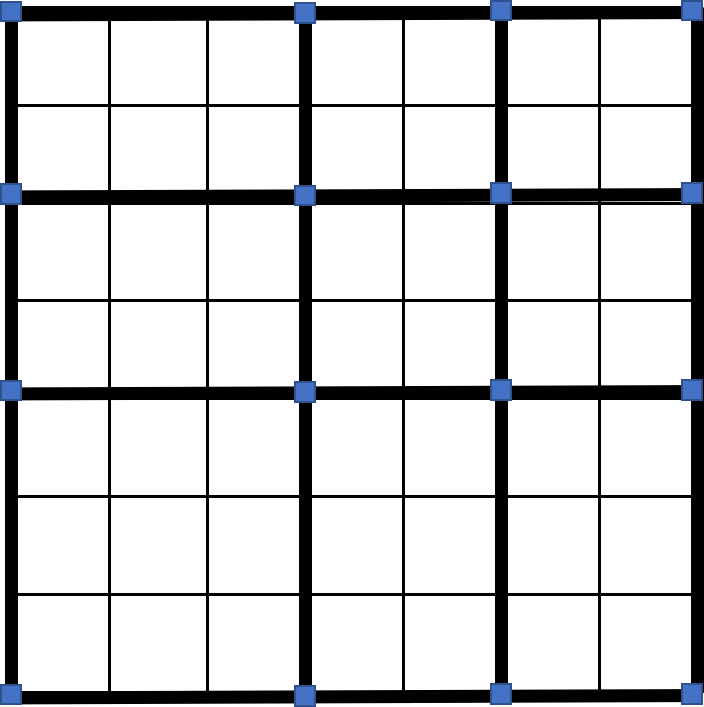
\includegraphics[width=6cm]{chap06/figs/grosso.png}
\caption{Exemplo de grid fino $7\time 7$ e um grid grosso $3\times 3$. O elemento inferior esquerdo é composto por 9 elementos do grid fino enquanto o elemento superior direito é composto com 4 elementos do grid fino.}
\label{fig:gridgrosso}

\end{figure}


No Capítulo \ref{ch:discretizacao} foi apresentada a discretização  para o problema de elasticidade linear através do método dos elementos finitos, com notação baseada em \cite{mbuck}. Naquele capítulo, a função desejada foi aproximada em um espaço $V^h$ formado por funções de base chapéu, no domínio $\Omega$ do problema. Agora vamos encontrar a solução do problema em um espaço grosso $V^{MS}$, tal que $V^{MS} \subset V^h$.



Para estabelecer o espaço $V^{MS}$, precisamos definir as suas funções de base geradoras.
Novamente, para distinguir o nó pertencente ao grid grosso dos seus graus de liberdade, o seguinte conjunto com graus de liberdade é criado:


\begin{equation}\label{eq:dheq}
    D^H = \{ p^{(m)} \in D^h : x^p \in \Sigma_H, m=1,2\}.
\end{equation}

\suge{acho que vc deveria esclarecer aqui cada um dos elementos da equação \eqref{eq:dheq}, mesmo que já tenha feito isso em algum capítulo anterior}


\begin{figure}[!htbp]
\centering
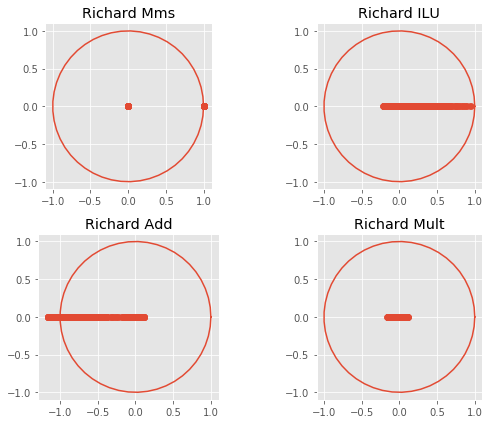
\includegraphics[width=11cm]{chap06/figs/IteracaoRichard.png}
\caption{Autovalores para matriz de iteração de Richard.}
\label{fig:nnzGrafico}
\end{figure}

\begin{figure}[!htbp]
\centering
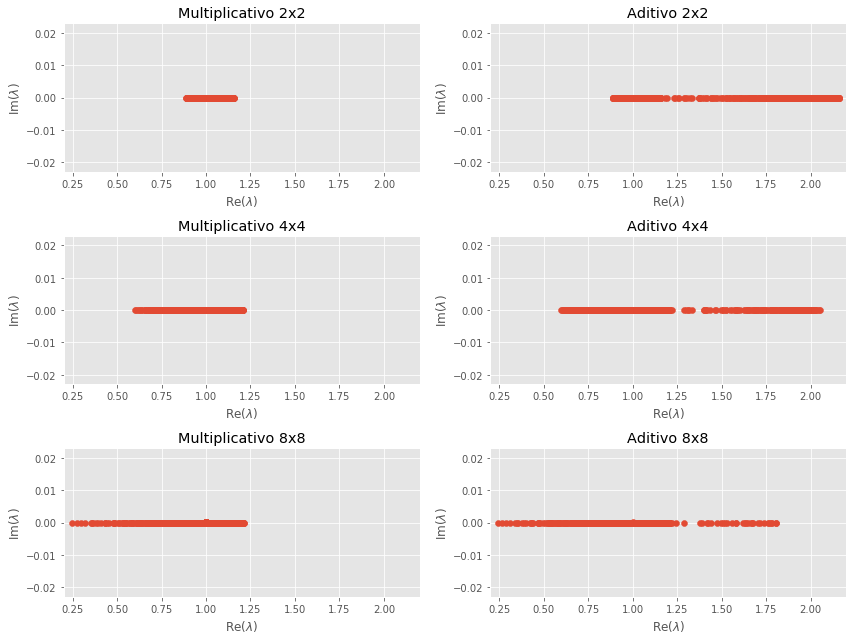
\includegraphics[width=11cm]{chap06/figs/AutovaloresMatPrecondicionada.png}
\caption{Autovalores da matrix pré-condicionada.}
\label{fig:nnzGrafico}
\end{figure}




\section{Cálculo do NNZ do operador de prolongamento}\label{sec:complexProlong}

Em um método multiescala, além da construção de um operador grosso,  precisa-se mover os vetores entre os espaços fino e grosso  Essas movimentações são realizadas através de multiplicação por operadores especiais, $P$ e $P^T$. Essa seção descreve a complexidade destas operações.

As dimensões do operador de prolongamento dependem dos graus de liberdade do operador fino e do  grosso, valendo $\qtdfreedomfine \times \qtdfreedomcoarse$. Conforme visto no Capítulo \ref{ch:sistemas}, a multiplicação de uma matriz esparsa por um vetor é da ordem do número de elementos  não nulos da matriz, assim, apesar de um maior engrossamento do grid reduzir o valor de $n_u^H$,  não necessariamente ocorre  uma redução de elementos não nulos de $P$. \suge{Talvez uma forma simples de motivar esta ideia, seja dizer que todos os elementos a matriz $A$ tem que ser multiplicados por algum elemento da matriz de restrição, não podendo ficar nenhum de fora, sendo assim, mesmo que ser reduza o número de linhas do operador de restrição, a quantidade de elementos não nulos não pode ser alterada. O que ocorre é que cada linha do operador de restrição, ou coluna do de extensão, fica mais densa quando se diminui a dimensão do espaço grosso}

Considerando um grid fino com $\numelementsxfine \times \numelementsyfine$, um grid grosso onde cada elemento tem dimensões $q_x \times q_y$ \suge{neste caso você está considerando que os elementos grossos são formados sempre pelo mesmo número de elementos, talvez seja o caso de dizer que você vai fazer isso mais lá em cima, apesar de isso não ser necessário} e, ainda, que mesmo os nós de fronteira com condição de contorno de Dirichlet não são removidos da matriz de rigidez, então a quantidade de não zeros do operador de prolongamento ($nnz_p$) pode ser calculada contando os nós de três conjuntos:  nós interiores, nós no vértice e os nós na aresta.  A Figura \ref{fig:gridCompleto} mostra cada um desse tipo de nós (em vermelho nó no vértice, em azul nó na aresta e em preto nó interior).


\begin{figure}[h]
\center
\subfigure[  ]{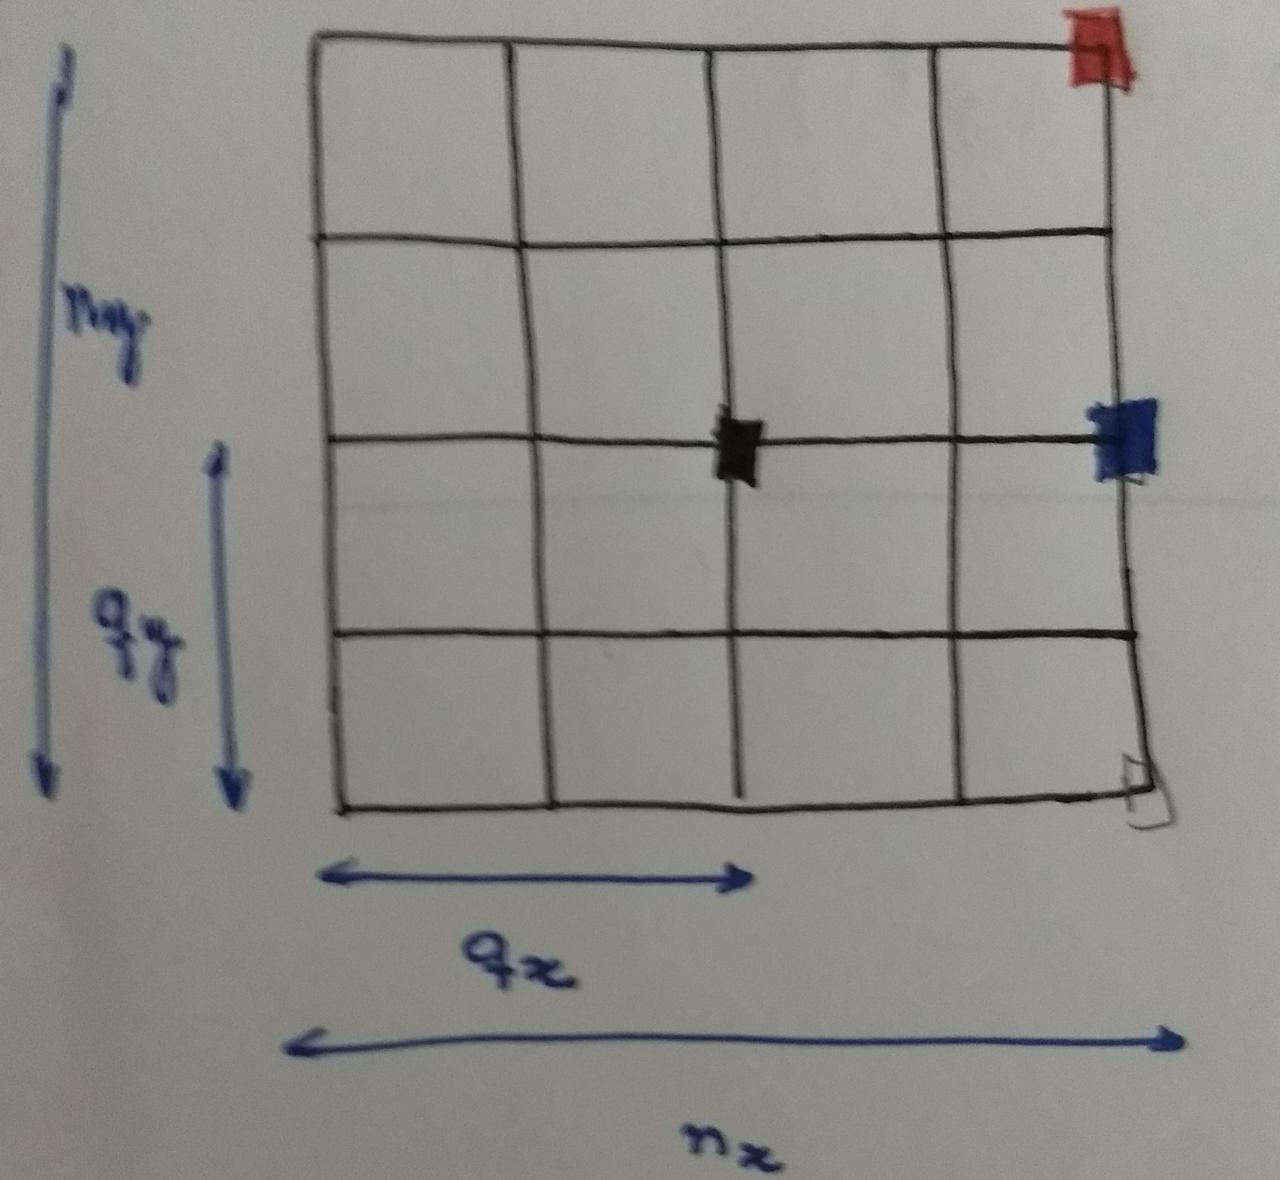
\includegraphics[width=0.45\textwidth]{chap06/figs/gridCompleto.jpeg}\label{fig:gridCompleto}}
\qquad
\subfigure[ ]{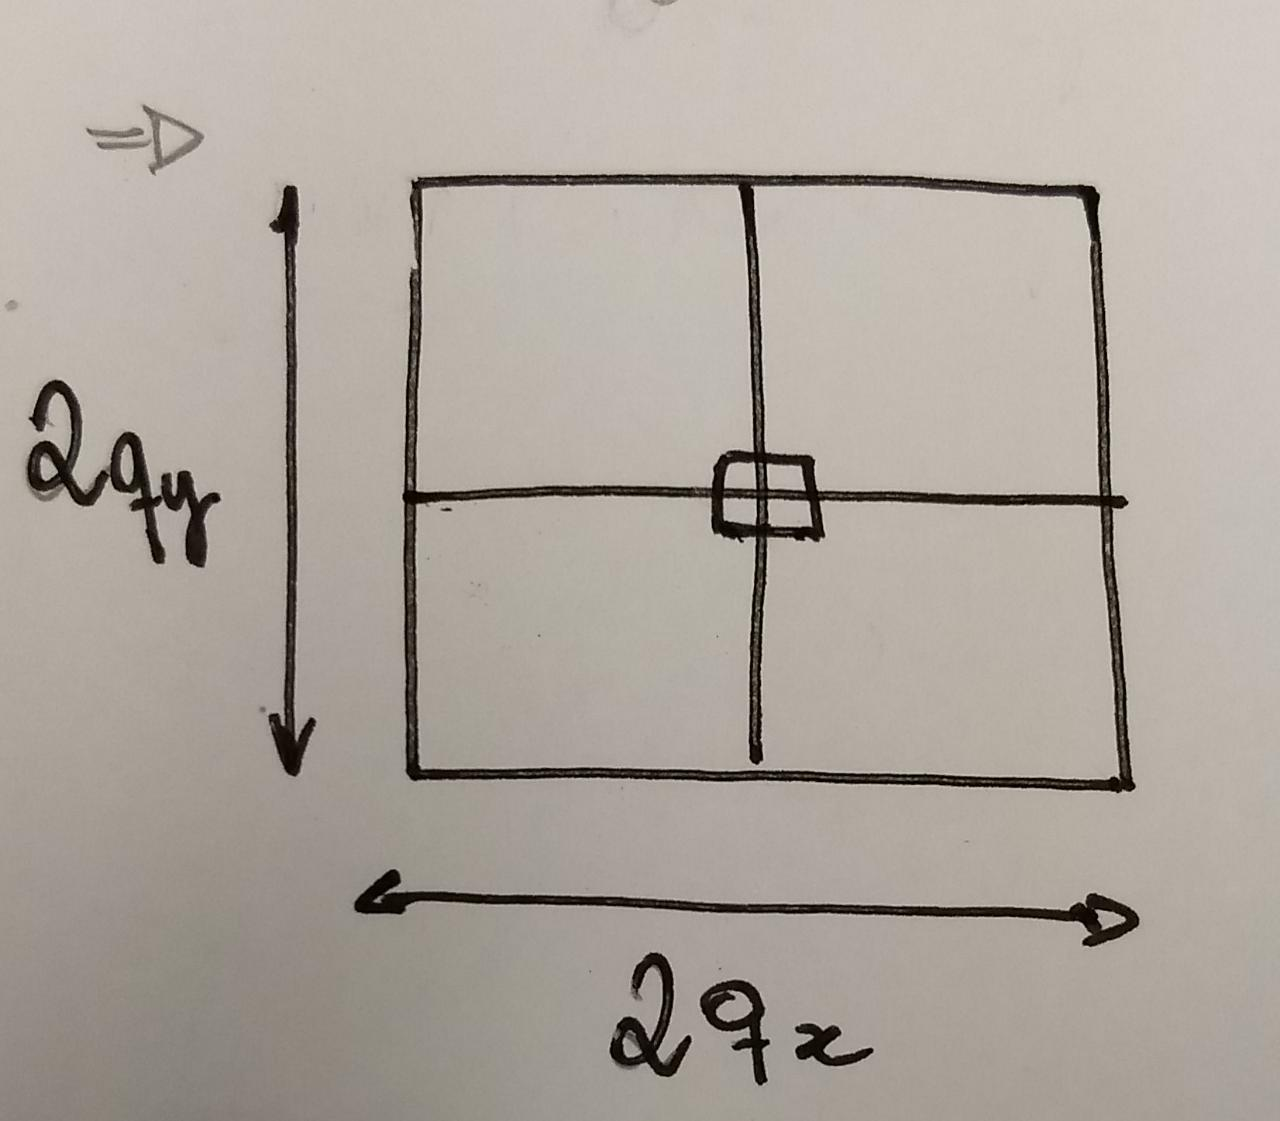
\includegraphics[width=0.45\textwidth]{chap06/figs/noInterior.jpeg}\label{fig:noInterior}}
\subfigure[ ]{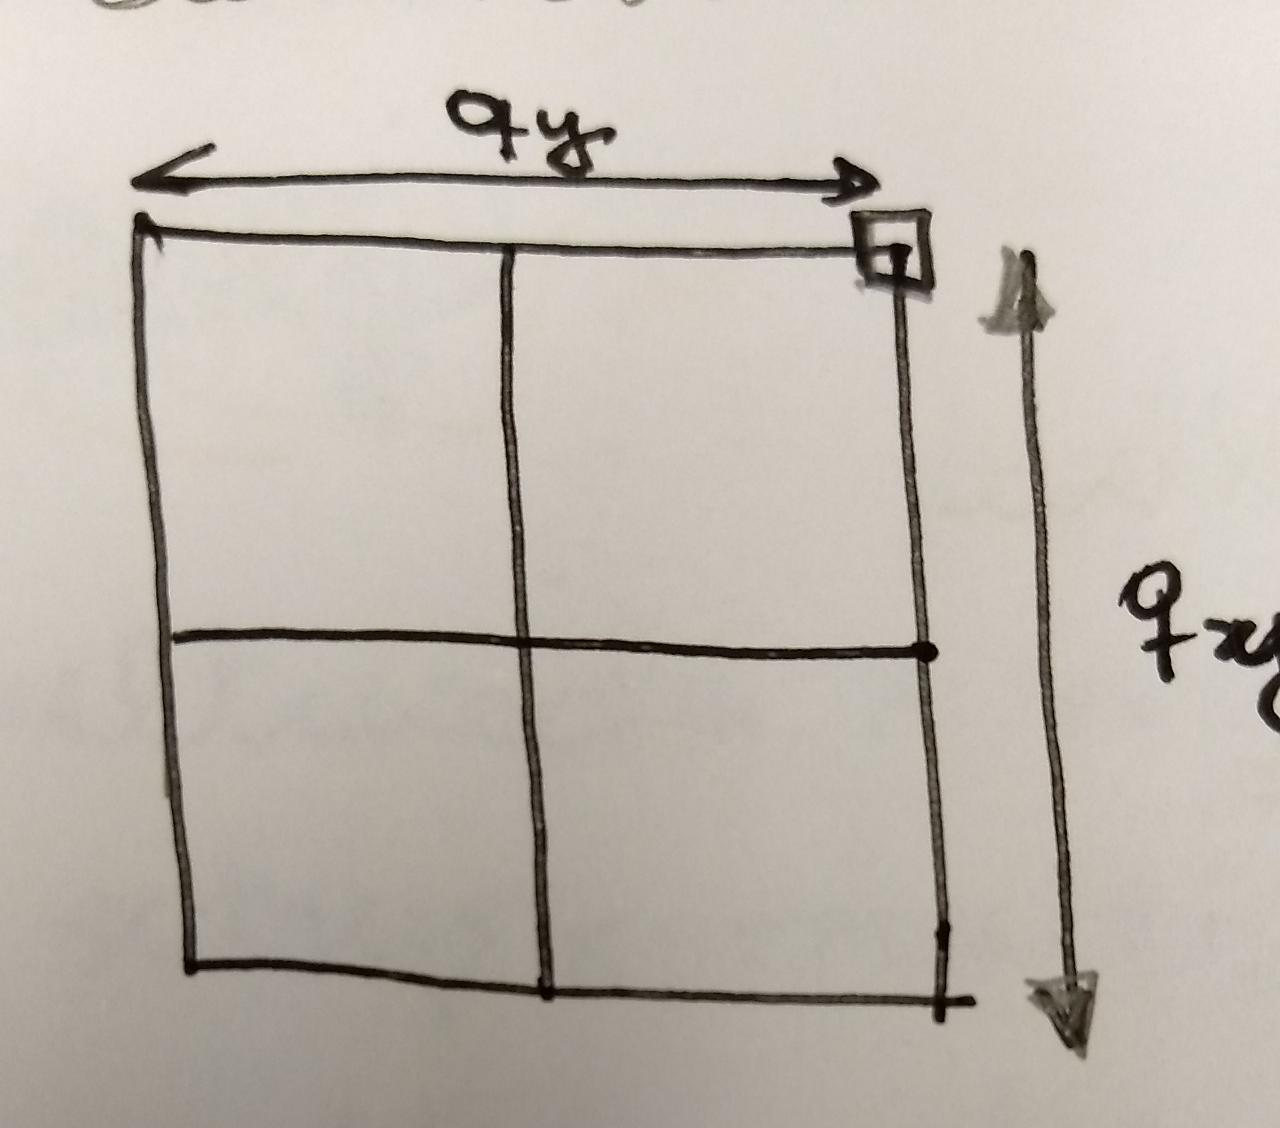
\includegraphics[width=0.45\textwidth]{chap06/figs/noVertice.jpeg}\label{fig:noVertice}}
\subfigure[ ]{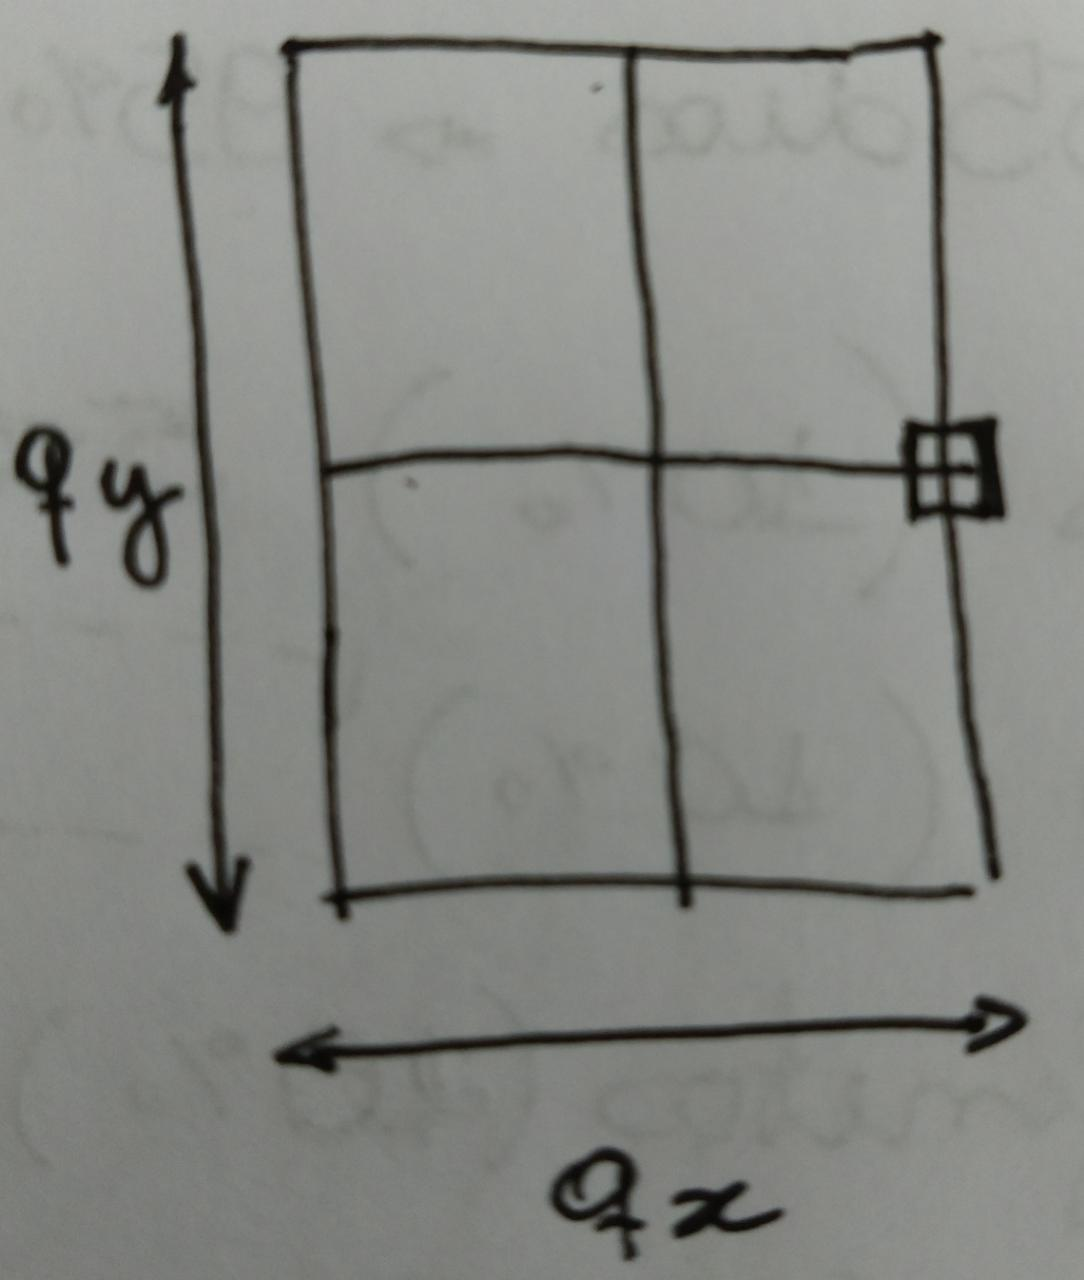
\includegraphics[width=0.45\textwidth]{chap06/figs/noAresta.jpeg}\label{fig:noAresta}}

\caption{Comparação da solução do grid fino com a solução do grid grosso.  }
\label{fig:verticesTypes}
\end{figure}

A quantidade de cada um desses nós na malha grossa é apresentado abaixo.

\begin{itemize}
    \item Nós interiores: $(\frac{n_x}{q_x} - 1) (\frac{n_y}{q_y} - 1)$
    \item Nós de aresta em $\Gamma_l$ e $\Gamma_r$: $2 ( \frac{n_y}{q_y} - 1)$
    \item Nós de aresta em $\Gamma_t$ e $\Gamma_b$: $2 ( \frac{n_x}{q_x} - 1)$
    \item Nós vértices: 4
\end{itemize}


Cada nó tem duas funções de base associadas uma para cada grau de liberdade (x e y). Para construirmos o operador de prolongamento que relaciona os nós do grid grosso com o fino, temos que a cada nó do grid grosso tem relação com $(2q_x+1)(2q_y+1)$ do grid fino. Este será o número de entradas não nulas que aparecerão em cada coluna do operador de prolongamento, como mostra a Figura \ref{fig:noInterior}. Além disso, ela afeta os dois graus de liberdade de cada um desses nós, então cada um deles contribui com $4(2q_x+1)(2q_y+1)$  não zeros para o prolongamento (uma implementação mais cuidadosa do método pode economizar as bordas do suporte pois as funções se anulam). De maneira análoga, os nós vértices contribuem com $ 4 (q_x+1)(q_y+1)$, os nós aresta em $\Gamma_t$ e $\Gamma_b$ contribuem com $ 4 (2q_x+1)(q_y+1) $ e, finalmente, os nós arestas  $\Gamma_l$ e $\Gamma_r$ e contribuem com $ 4(q_x+1)(2q_y+1) $. Assim, para encontrar a quantidade total de não zeros do operador de prolongamento, basta multiplicar as quantidades de cada um dos nós pela duas contribuições conforme a   \eqref{eq:nnzRaw}.


\begin{equation} \label{eq:nnzRaw}
\begin{aligned}
    nnz_P = & 4(2q_x+1)(2q_y+1)  (\frac{n_x}{q_x} - 1) (\frac{n_y}{q_y} - 1)   \\
            & + 4 (q_x+1)(2q_y+1)  2 ( \frac{n_y}{q_y} - 1) +  4 (2q_x+1)(q_y+1)  2 (\frac{n_x}{q_x} - 1) \\
            & +  4(q_x+1)(q_y+1) 4
\end{aligned}
\end{equation}

Que pode ser modificada para a \eqref{eq:nnzRaw2},

\begin{equation} \label{eq:nnzRaw2}
\begin{aligned}
    nnz_P = &   4 (2+\frac{1}{q_x})(2 + \frac{1}{q_y})  (n_x - q_x) (n_y - q_y) \\
            & + 8 (q_x+1)(2 + \frac{1}{q_y})  (n_y - q_y) \\
            & + 8 (2+\frac{1}{q_x})(q_y+1) (n_x - q_x) \\
            & + 16 (q_x+1)(q_y+1)
\end{aligned}
\end{equation}

Assim, se $q_x$ e $q_y$ são de ordem $O(1)$ o primeiro termo da soma é da ordem de $O(n_x \times n_y)$. Caso $q_x$ e $q_y$ sejam de ordem $O(n_x)$ e $O(n_y)$, então o último termo da soma é da ordem $O(n_x \times n_y )$. \suge{não vejo muito sentido em $q_x$ ser $O(1)$, pois $q_x$ e $n_x$ vão sempre ter uma relação direta e, neste caso, o conceito de ordem esconde a constante de proporcionalidade e não ajuda a definir bem a complexidade do problema. $q_x$ e $n_x$ não teriam relação caso um fosse fixado e outro alterado, que é a situação mostrada na Figura \ref{fig:nnzGrafico}}
Se $q_x$ é $O(n_x)$ e $q_y$ é $O(1)$ então o segundo termo é de ordem $O(n_x \times n_y)$, analogamente para o caso contrário.
De toda forma, a quantidade de não zeros do prolongamento é da ordem do tamanho do grid $n_x \times n_y$ que é um fato importante, pois a multiplicação pelo prolongamento faz parte do processo de utilização do pré-condicionador multiescala e esse preço sempre terá que ser pago. O valor limite também dos não zeros é representado pelo último termo da soma $16(q_x+1)(q_y+1)$.

Um gráfico representando    \eqref{eq:nnzRaw2} é mostrado na Figura \ref{fig:nnzGrafico}, no eixo y é apresentado $nnz_P$ enquanto no eixo x é apresentado o engrossamento da malha que tem a mesma proporção em x e y ($q_x  = q_y$) para um grid de $1024 \times 1024$. Pelo gráfico é possível ver que o $nnz_P$ tende já em um engrossamento $16 \times 16$.


\begin{figure}[!htbp]
\centering
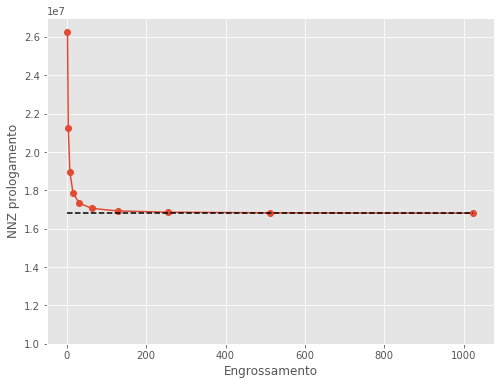
\includegraphics[width=8cm]{chap06/figs/nnzProlongamento.png}
\caption{Quantidade de não zeros do prolongamento $nnz_P$  em função do engrossamento da malha. A linha pontilhada mostra o valor de $16(n_x+1)(n_y+1)$.}
\label{fig:nnzGrafico}
\end{figure}
